\documentclass{article}
\usepackage[utf8]{inputenc}
\usepackage{algorithm}
\usepackage{algorithmic}
\usepackage{amsthm}
\usepackage{graphicx}
\theoremstyle{definition}
\newtheorem{definition}{Definíció}
\title{Szakdolgozat}
\author{Szabó Bence Dániel }
\date{Date}

\begin{document}

\maketitle

\section{Lineáris egyenletrendszerek megoldása}


A matematika rengeteg egyenlet megoldásán alapszik. Ezeknek az egyenleteknek a legegyszerűbb formái a lineáris egyenletek és egyenlet rendszerek. Ezeket könnyű megoldani papíron, mert nem igényel nagy módszertani tudást. Azonban előfordul sok esetben, hogy már nem optimális papíron megoldani ezeket az egyenleteket, mert nagyon igényes a kiszámolása és a sok apró művelet során könnyen hibára futhatunk, amit jó eséllyel észre sem vennénk. 

Legyen A $\in \mathbb{R}^{n x n}$ egy valós mátrix, b $\in \mathbb{R}^{n}$ egy valós vektor és x $\in \mathbb{R}^{n}$ egy olyan vektor, ami kielégíti a következő egyenlőséget.
\begin{center}
    $Ax = b$
\end{center}
Célunk az x vektor kiszámolása. Természetesen x vektort megkaphatjuk egy mátrix invertálás majd szorzás után:
\begin{center}
    $x = A ^{-1}b$
\end{center}
Azonban most nem az invertálást nézzük meg, hanem a Gauss eljárást. A Gauss eljárás úgy működik, hogy fentről lefelé ellenőrizve a sorokat mindig kiejtünk egy ismeretlen, a legvégén pedig egyértelműen kapunk egy ismeretlen - konstans párost. Ekkor pedig meghatározzuk az első ismeretlent, onnan a következő sorban behelyettesítjük az elöző lépésben megkapott ismeretlent és megint egyértelműen meghatározható a következő ismeretlen. Ezt pedig addig folytatjuk, amíg nincs meg a teljes x vektor. A következőben a Gauss eljárás egyik pszeudo kódját láthatjuk. Természetesen, ha az átlóban 0 elem kerül, akkor hibára futunk. A gyakorlatban azért, mert 0-val nem tudunk osztani, klasszikus matematikai értelemben azért, mert nem lesz megoldható az egyenletrendszer.

\begin{algorithm}
%http://www.math-cs.gordon.edu/courses/ma342/handouts/gauss.pdf
\caption{Gauss eljárás}
\begin{algorithmic}
\STATE INPUT: A együttható mátrix utolsó oszlopában az egyenletek értékeivel
\STATE OUTPUT: x megoldás vektor
\STATE n: A és b sorainak száma
\FOR{$(k = 1,k < n - 1 ; k ++$)} 
\FOR{$(i = k + 1,k < n ; i ++$)}
\STATE $a_{ik} = a_{ik} / a_{kk}$
\FOR{$(j = k + 1,k < n ; j ++$)} 
\STATE $a_{ik} = a_{ij} - a_{ik} a_{kj}$
\ENDFOR 
\ENDFOR 
\ENDFOR 

\FOR{$(k = n , k > 1 , k--)$}
BALANCE(a_{k,})
\newline
$ x_i = SUM(a_{k,})$
\ENDFOR
\end{algorithmic}


\end{algorithm}
\newpage
\section{Numerikus integrálás}
A numerikus integrálás nagyon fontos része a numerikus módszereknek. Egyrészről gyorsabban megkaphatjuk a határozott  integrál értékét, másrésszről vannak olyan függvények, amelyeknek nem tudjuk kiszámolni papíron az integrál értéket, csak becsülni tudjuk alulról és/vagy felülről.

\begin{definition}
Lagrange-féle interpolációs polinom

Ezt még meg kell írni + nézd meg az opkut3-as dolgokat!
\end{definition}
A numerikus integrálás nagyban támaszkodik a kvadratúra képletekre.
\begin{definition}
Kvadratúra képletek általánosan

Az integrál értékét tudjuk közelíteni az ún. \textit{Kvadratúra képlettel}. 
\newline
$\int_{a}^{b} f(x) dx \approx \sum_{k = 0}^{n} c_k f(x_k) = \sum_{k=0}^n \sigma_k$ , ahol $x_i \in [a,b]$
\end{definition}

Most nézzünk meg néhány kvadratúra képletet.
\subsection{Newton - Cotes formula}


Az integrálni való halmazt osszuk fel egyforma hosszúságúra, így vegyünk ekvidisztáns alappontokat.
$x_k = a + hk $, ahol $k=0,1,...,n$ , $h = \frac{b-a}{n}$

Írjuk fel az interpolációs kvadratúra képletet.
\newline
$c_k = \int_a^{b} l_k(x) dx = h \int_0^{n} l_k (a+ht) dt = \frac{b-a}{n} \int_0 ^{n} \Pi_{j=0, j \neq k}^n \frac{t-j}{k-j} dt = \frac{b-a}{n} \frac{1}{k! (n-k)!} \int_0^n \Pi_{j=0}^{k-1} (t-j) \Pi_{j=k+1}^{n} (j-t) dt$


\subsection{Összetett kvadratúra képlet}

\begin{center}
 $\int_a^{b} f(x) dx = \sum_{j = 1} ^{m} \int_{a_{j-1}} ^{a_j} f(x) dx$ , ahol $a_0 = a, a_m =b$   
\end{center}


A baloldali részintegrált írjuk fel az interpolációs kvadratúra képlettel:
\begin{center}
$\int_{a_{j-1}}^{a_j} f(x) dx \approx \sum_{k=0}^{r} c_{k,j}f(x_{k,j})$
\end{center}

Innen helyettesítsünk vissza az eredeti képletbe
\begin{center}
$\int_a^b f(x) dx \approx \sum_{j=1}^{m} \sum_{k=0}^{r} c_{k,j} f(x_{k,j})$
\end{center}


\subsection{Érintő formula}

Az érintő formulához felfogjuk használni a függvények lineáris Taylor közelítését. Ezen felül vegyük az intervallum ekvidisztáns felosztását.
\begin{center}
   $x_k = a + (k - \frac{1}{2})h$ , ahol $h = \frac{b-a}{n}, k =1,...,n$ 
\end{center}
A Taylor közelítése a függvénynek az $[x_k-\frac{h}{2},x_k+\frac{h}{2}]$ :
\begin{center}
   $f(x) \approx f(x_k)+f'(x_k)(x-x_k)$ 
   Ezt felhasználva
$\int_{x_k - \frac{h}{2}}^{x_k + \frac{h}{2}} \approx \int_{x_k - \frac{h}{2}}^{x_k + \frac{h}{2}} [f(x_k) + f'(x_k)(x-x_k)] dx = hf(x_k)$

Innen pedig kapjuk, hogy
$\int_a^b = f(x) dx = \sum_{k=1}^n \int_{x_k - \frac{h}{2}}^{x_k + \frac{h}{2}} f(x)dx \approx h \sum_{k=1}^n f(x_k)$
\end{center}

\textbf{Ide rakd be az érintős-integrálós rajzot}

\subsection{A trapéz módszer és a Newton - Cortes módszer}
Írjuk fel a Newton - Cortes formulát n = 1 és k = 0 melett:
\begin{center}
$c_0 = \frac{b-a}{1} \frac{1}{0!(1-0)!} \int_0^{1} \Pi_{j=0}^{0-j} \Pi_{j=0+1}^{1} (j-t) dt = (b-a) \int_0^1 (1-t) dt = \frac{b-a}{2}$
\end{center}

\begin{center}
$c_1 = \frac{b-a}{2}$
\end{center}
Ekkor 

\begin{center}
    $\int_a^b f(x) dx \approx \frac{b-a}{2}[f(a) + f(b)] = \sum_{k=0}^{1} \frac{b-a}{2} f(x_k)$, ahol $x_0 = a,x_1=b$
\end{center}
Ez pedig pont a trapéz területe!
\newline

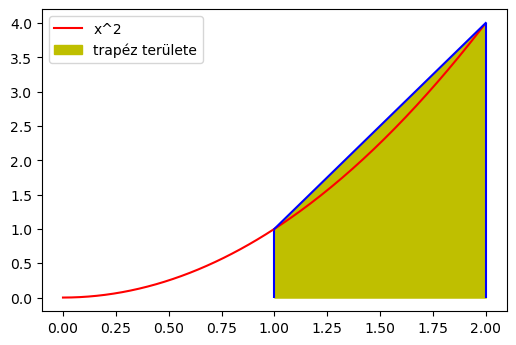
\includegraphics{plots/trapez_with_area.png}

ötlet : rakd bele ,hogy az integrál 7/3 itt de ez most 2.5-t ad . Ezt látni,hogy a trapéz teteje a vonal fölött van. Ezután osszd fel 2,3,4,... részre és számold ki ezzel a területet.
\begin{definition}
Legendre polinom
[...]
\end{definition}
\begin{definition}
Gauss - féle kvadratúra összegek
\end{definition}

\subsection{Python kódok a fejezethez (saját , legyeb SciPy?)}

\subsection{Feladatmegoldások}
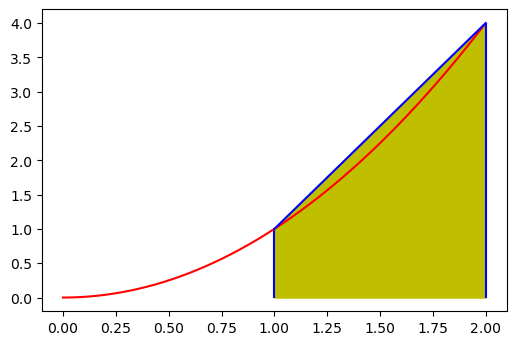
\includegraphics{plots/Unknown.png}
\end{document}
